\documentclass{article}
\usepackage[T2A]{fontenc}
\usepackage[utf8]{inputenc}
\usepackage[english,russian]{babel}
\usepackage{listings} 
\lstset{language=Python}

\usepackage{amsmath}

\usepackage{graphicx}
\graphicspath{ {images/} }

\title{ Статические и эмперические методы компьютинга}
\author{Арбузов Ф. П. БПИ151}
\date{Февраль 2017}

\begin{document}
\maketitle
\setlength{\parindent}{0cm}

\section*{Задача 1}
\section*{Пункт а}
Сгенерируйте выборку объёма 100 из распределения, соответствующего вашему варианту. Постройте гистограмму с 10 столбцами для полученной выборки.Сгенерируйте выборку объёма 1000 из того же распределения и постройте гистограмму с 10 столбцами для неё. Сравните с ранее полученным графиком. Если графики различаются, попробуйте описать и объяснить различия.


\section{Генерируем рандомную выборку:}
\begin{lstlisting}[frame=single]   % Start your code-block

from math import *
from random import random

def f(p):
    i = log((1/e - 1)*(p - (1/(1 - 1/e))), e)
    return -1 * i

data = []
for i in range(0, 100):
    r = random()
    if (r == 0): r = random()
    data.append(f(r))

print("NOW DATA:")
print(["{:.3f}".format(n) for n in data])

\end{lstlisting}
Набор случайных чисел
\[

'0.493', '0.931', '0.882', '0.310', '0.244', '0.089', '0.034', '0.100', '0.588', '0.635', '0.688', '0.884', '0.006', '0.977', '0.256', '0.115', '0.111', '0.017', '0.294', '0.019', '0.613', '0.255', '0.182', '0.207', '0.900', '0.265', '0.336', '0.394', '0.254', '0.198', '0.730', '0.179', '0.510', '0.079', '0.630', '0.232', '0.664', '0.248', '0.033', '0.679', '0.591', '0.092', '0.870', '0.052', '0.467', '0.540', '0.239', '0.280', '0.244', '0.784', '0.643', '0.301', '0.023', '0.198', '0.474', '0.399', '0.879', '0.997', '0.042', '0.126', '0.182', '0.599', '0.740', '0.389', '0.003', '0.128', '0.119', '0.297', '0.959', '0.015', '0.224', '0.370', '0.394', '0.738', '0.117', '0.905', '0.740', '0.164', '0.689', '0.231', '0.374', '0.695', '0.525', '0.502', '0.358', '0.837', '0.335', '0.128', '0.106', '0.088', '0.101', '0.118', '0.474', '0.075', '0.072', '0.074', '0.322', '0.617', '0.036', '0.688'


 

\]


\section{Получим функцию квантилей}
Функция распределения:

\[
 F(x) = 
  \begin{cases} 
   \ 0 & \text{if } x < 0 \\
   \ \frac{(1 - e^{-x})}{(1 - e^{-1})} & \text{if } 0 < x < 1 \\
   \ 1 & \text{if } x < 0
  \end{cases}
\]
Тогда функция квантилей:
\[
 Q(x) = -\ln{((\frac{1}{e} - 1)(p - \frac{1}{1 - \frac{1}{e}}))}
\]

\section{Таблица статистического ряда}
\begin{tabular}{| r | r | r | r | r | r | }
  \hline			
Интервал & '0.00,0.10' & '0.10,0.20' & '0.20,0.30' & '0.30,0.40' & '0.40,0.50' \\
Частота & 0.2 & 0.15 & 0.16 & 0.11 & 0.04\\
  \hline  
\end{tabular}

\medskip

\begin{tabular}{| r | r | r | r | r | r | }
  \hline			
Интервал & '0.50,0.60' & '0.60,0.70' & '0.70,0.80' & '0.80,0.90' & '0.90,1.00'\\
Частота & 0.07 & 0.11 & 0.05 & 0.05 & 0.06\\
  \hline  
\end{tabular}

\section{Гистограмма}



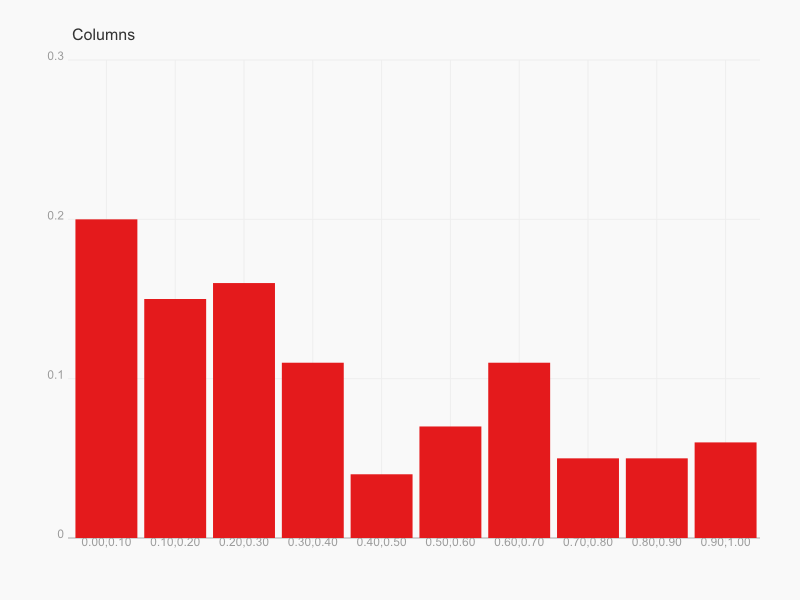
\includegraphics[scale=0.7]{columns.jpg}

Для выборки объема 100

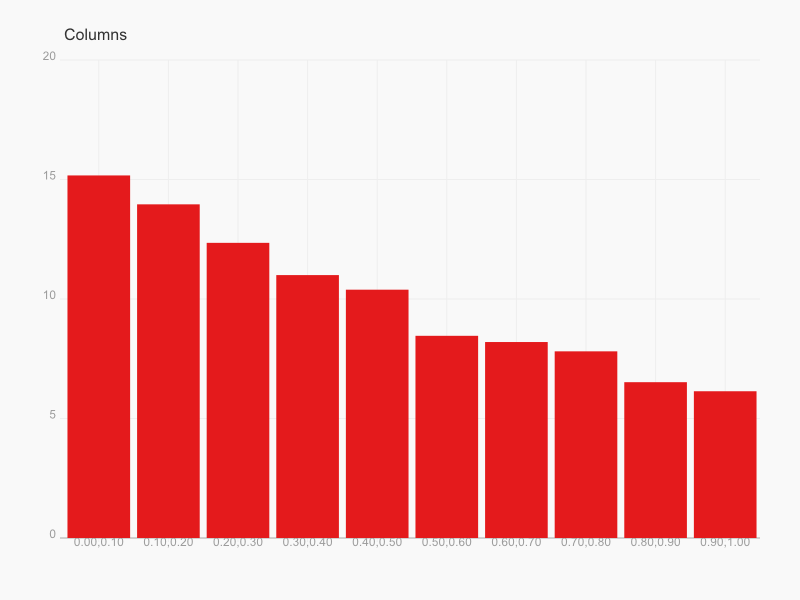
\includegraphics[scale=0.7]{columns(1).jpg}

Для выборки объема 1000

\section*{Пункт б}
Сгенерируйте выборку, состоящую из 1000 реализаций случайных величин
$$Y_{i} = \sum_{j=1}^{30} X_{ij}, i = 1..1000 $$,
где $$ X_{ij} $$ – независимые случайные величины с распределением, соответствующим вашему варианту. Постройте гистограмму для полученных данных, сравните её с графиками из пункта (а).
\end{document}
